\documentclass[12pt]{article}
\usepackage{geometry}
\geometry{letterpaper, left=22.5mm, right=22.5mm, top=30mm, bottom=30mm}
\geometry{letterpaper}
\usepackage{amsmath}
\usepackage{amssymb}
\usepackage{enumitem}
\usepackage{fancyhdr}
\usepackage{framed}
\usepackage{tikz}
\usepackage{mathpazo}
%\usepackage{charter}
%\usepackage{newcent}
\usepackage{indentfirst}
\usepackage{booktabs}
\usepackage{graphicx}
\usepackage{float}
\usepackage{makecell}
\usepackage{xcolor}
\usepackage{mdframed}
\usetikzlibrary{trees}
\pagestyle{fancy}
\usepackage{amsthm}
\theoremstyle{definition}
\newtheorem{definition}{Definition}[section]
\theoremstyle{property}
\newtheorem{property}{Property}[section]
\theoremstyle{assumption}
\newtheorem{assumption}{Assumption}[section]
\theoremstyle{example}
\newtheorem{example}{Example}[section]
\theoremstyle{comment}
\newtheorem{comment}{Comment}[section]
\newtheorem{theorem}{Theorem}[section]
\newtheorem{corollary}{Corollary}[theorem]
\newtheorem{lemma}[theorem]{Lemma}
\usepackage{lastpage}
\usepackage{wrapfig}
\usepackage{hyperref}
\usepackage{subcaption}
\usepackage{setspace}
\hypersetup{
colorlinks=true,
linkcolor=black,
filecolor=green, 
urlcolor=blue,
}
\newcommand{\ROM}[1]
    {\MakeUppercase{\romannumeral #1}}
    
    \DeclareMathOperator*{\plim}{plim}
\fancyhead[L]{Econometrics \ROM{2}: Recitation 11}%change each reci
\fancyhead[R]{Spring 2022}
\fancyfoot[C]{\thepage \hspace{1pt} / \pageref{LastPage}}

\fancypagestyle{firstpage}{%
\fancyhf{}%
\renewcommand{\headrulewidth}{0mm}%
  \fancyfoot[C]{\thepage \hspace{1pt} / \pageref{LastPage}}
}
%change title each rec
\title{Introduction to Econometrics \ROM{2}: Recitation 11}

\begin{document}
\linespread{1.25}
\onehalfspacing

\author{Seung-hun Lee\footnote{Contact me at \href{mailto:sl4436@columbia.edu}{sl4436@columbia.edu} if you spot any errors or have suggestions on improving this note.}}
\date{April 18th, 2022}
\maketitle
\thispagestyle{firstpage}

%%%%%%%%%%%%%%%%%%

\section{Treatment Effects}


\subsection{Difference-in-Difference Estimation}
This involves a specific framework where we can clearly define a `before and after' - denoted as $t_0$ and $t_1$. For now, we assume that there are just these two periods. No one is treated at $t_0$ but there is a subset of people ($G_i=1$) that are treated at $t_1$. Those in $G_i=0$ are never treated in either time period. If we define a framework similar to our cross-sectional potential outcomes as
\[
y_{i,t}=G_iy_{i}(1,t)+(1-G_i)y_{i}(0,t) \ \ (t\in\{t_0, t_1\})
\]
then we will be able to observe $(y_{i,t_1}, y_{i,t_0},G_i, X_i)$ for every unit $i$. What we do not observe is $y_i(1,t_1)$ for those in $G_i=0$ and $y_i(0,t_1)$ for those in $G_i=1$, similar to the fundamental problem of missing data for our cross-sectional potential outcome framework. The analogue to the conditional independence assumption is a \textbf{parallel trend assumption}, defined as
\[
(y_i(1,t_1)-y_i(1,t_0), y_i(0,t_1)-y_i(0,t_0)) \perp\!\!\! \perp G_i|X_i
\]
Using the fact that no one is treated in $t_0$, we can skip $G_i$ notation for $t_0$ and write  $y_i(G_i,t_0)=y_i(t_0)$ for $G_i\in\{0,1\}$ and write the above condition as  
\[
(y_i(1,t_1)-y_i(t_0), y_i(0,t_1)-y_i(t_0)) \perp\!\!\! \perp G_i|X_i
\]\par
Both versions of the parallel trend assumption imply that the changes in treatment outcome for both groups do not depend on $G_i$ once we condition for $X_i$. This would be violated if uncontrolled factors affect the changes in the outcome or if there are differences in the trends of $y_{i,t}$ across treated and control groups even before the experiment. \par
To see why they are equal, consider a setting where $D_i=G_i$ and write
\begin{align*}
y_i = y_{i,t_1}-y_{i,t_0}&=D_i(\underbrace{y_i(1,t_1)-y_i(1,t_0)}_{y_i(1)})+(1-D_i)(\underbrace{y_i(0,t_1)-y_i(0,t_0)}_{y_i(0)})\\
&=D_iy_i(1) + (1-D_i)y_i(0)
\end{align*}
Thus, we can write the parallel trend assumption as conditional independence assumption. 
\[
(y_i(1), y_i(0)) \perp\!\!\! \perp D_i|X_i
\]
\par
To apply this in regression, we can write
\[
y_{it}=\beta_0(X_i)+\beta_1(X_i)\cdot\mathbb{1}[t=t_1]+\beta_2(X_i)\cdot G_i + \beta_3(X_i)\cdot G_i\cdot\mathbb{1}[t=t_1]+\epsilon_{it}
\]
where $X_i$ is a set of covariates, which can include a constant. In this context, the treatment effect for $X_i=x$ would be
\begin{align*}
TE(x)&=E[y_i(1)-y_i(0)|X_i=x]\\
&=E[(y_i(1,t_1)-y_i(1,t_0))-(y_i(0,t_1)-y_i(0,t_0))|X_i=x]\\
&=x\cdot E[\{(\beta_0+\beta_1+\beta_2+\beta_3)-(\beta_0+\beta_2)\}-\{(\beta_0+\beta_1)-(\beta_0)\}|X_i=x]\\
&=x\cdot E[(\beta_1+\beta_3)-\beta_1|X_i=x]\\
&=\beta_3 x
\end{align*}
So $\beta_3$ would be our parameter of interest. \par
One difficulty arises from testing the parallel trends assumption. Loosely speaking, what we can do is to select a time period $\tilde{t}<t_0$ and find out if the difference $y_i(t_0)-y_i(\tilde{t})$ is independent with $G_i$. If not independent, we say that there is an pre-trend. This is why when difference-in-difference is presented, many researchers also plot the pre-treatment outcome. This does not perfectly test parallel trends, as plotting the coefficients does not perfectly take into account the influence of unobserved factors that may violate parallel trends. However, if there are noticeable trends pre-treatment, that is a sure sign of nonparallel trends. 
\subsection{Two-way fixed effects}
For a setup with just two time periods, running a difference-in-difference is equivalent to
\[
y_{it}=a_i+b_t + cD_{it}+e_{it}
\]
where $D_{it}=1$ if unit $i$ is treated at period $t$ and $0$ if otherwise. We extend the simple difference-in-difference model by including more time periods and allowing absorbing treatment where individuals enter the treatment at different time and stay treated afterwards. In other words, if $D_{it}=1$, then for $\tau>t$, $D_{i\tau}=1$. \par
While the implementation is simple, there may be problems. There may exist a compositional effect where the overall trend in the data is reversed or attenuated compared to a trend that appears in the groups composing the data. The consequence is that in the case where there is a strong heterogeneity of treatment across groups or time, the coefficient of $c$, which is are treatment effect variable, may end up with the opposite sign of a true effect. \par
To see why this can happen, we need to understand that the estimate of $c$ is a weighted average of various $i\times t$ cells\footnote{Among many DiD papers, the most straightforward explanation comes from Goodman-Bacon (2021 Journal of Econometrics) and Jakiela (2021, WP)}. Let $G_i$ be the first period in which $i$ is treated. If $i$ is never treated, let $G_i=\infty$. By applying (two-step) within estimation, we can get
\[
\hat{c} = \frac{\sum_{i.t}\tilde{y}_{it}\widetilde{D}_{it}}{\sum_{i.t}\widetilde{D}_{it}^2}
\]
where $\tilde{y}_{it}=y_{it}-\bar{y}_{i\cdot}-\bar{y}_{\cdot t}+\bar{y}$ and similarly for $\widetilde{D}_{it}$. Other way to see this is to apply the Frisch-Wald-Lovell theorem: We get the same estimate by regressing $y_{it}$ onto the residual of 
\[
D_{it} = a_i+b_i+u_{it} 
\]
In this way, we can write
\[
\hat{c}=\frac{\sum_{i,t}y_{it}\hat{u}_{it}}{\sum_{i,t}\hat{u}_{it}^2}=\sum_{i,t}y_{it}\left(\frac{\hat{u}_{it}}{\sum_{i,t}\hat{u}_{it}^2}\right)
\]
Thus, you can see that $\hat{c}$ is a weighted sum of the values of the outcome variable across various $i\times t$ cells. Theoretically, each $i\times t$ has a different weight and some observations end up getting \textit{negative} weights. This happens since $\hat{u}_{it}$ is not necessarily binary, and those whose treatment intensity is below the mean gets negative weights. These are usually the early adopters in later years (high unit-level treatment mean and time-level treatment mean) that are practically treated as comparison group to the recently treated group.  
\par
To deal with this, the minimum requirement is to vary the coefficient $c$ across different time by letting it differ by the implementation period, $c(G_i)$. This is usually not enough, however. The best approach is to compare the average treatment effect for those treated at a earlier period vs. those that are treated later. Specifically, for a specific $g\leq t$,  and for any $g'>t$, write
\[
E[y_{it}(g)-y_{it}(\infty)|G_i=g]=E[y_{it}-y_{i,g-1}|G_i=g]-E[y_{it}-y_{i,g-1}|G_i=g']
\]
In this way, we are not making a wrongful comparison against the early-adopters. Also, it is nicer to have those who are never treated (pure control) since they always serve as a safe comparison group. 
\subsection{Violation of Conditional Independence Assumptions}
There are cases where the assignment, even if we condition on observables, are not random. So in the regressional framework of $y_{i}(d)=\mu(X_i,d)+\epsilon_i(d)$, the error terms is not independent of $D_i|X_i$. The conditional independence assumption can be broken because:
\begin{itemize}
\item Participants self-select based on expected benefit: Think about a job training program for plumbing. Then, maybe those who are more healthy and suffer less in terms of costs are likely to join. If health is not perfectly observed, we risk breaking the conditional independence assumption
\item Participants may be selected, consciously or not, to join: Think of the clinical trial where participation is voluntary. In such case, individuals who are more risk-loving are more likely to join. In other words, participants and nonparticipants systematically differ on risk-averseness - something that is not usually observed.
\item There may be equilibrium effects: A tuition subsidy program that intends to increase the number of people entering college may have a spillover effect by increasing supply of college graduates at the labor market, leading to a decrease in college premium. This may induce students to enter college less. If TE is the (rate of) college entrance, such equilibrium effect may be influential.  
\end{itemize}
\par
Mathematically, what happens is that when we calculate $E[y_i|D_i=1,x]-E[y_i|D_i=0,x]$, we end up with
\begin{align*}
E[y_i|D_i=1,x]-E[y_i|D_i=0.x]&=\mu(x,1)-\mu(x,0)+E[\epsilon_i(1)|D_i=1,x]-E[\epsilon_i(0)|D_i=0,x]\\
&=TE+\underbrace{E[\epsilon_i(1)|D_i=1,x]-E[\epsilon_i(0)|D_i=0,x]}_{\text{(Positive/Negative) selection bias}}
\end{align*}
The error term no longer can be erased from the equation since CIA assumption is not applicable. The difference between the error term is the \textbf{selection bias} that can be both negative and positive (Also appears in Angrist, Pischke 2009). This also means that the error terms $(\epsilon_i(1), \epsilon_i(0))$ and the $u_i$ in $D_i=\mathbb{1}[u_i<p(x_i)]$ can covary. The result is that the treatment effect estimated from here can be inaccurate. \par
There are two possible solutions. Old method relies on \textbf{Heckman correction}. Recent focus is on IV to derive \textbf{marginal treatment effects} and \textbf{localized average treatment effect}.
\subsection{A Brief Discussion of the Heckman Correction}
Suppose that we are in the situation where we have a data generating process
\[
y_i = \max\{X_i\beta+\sigma\eta_i, 0\}, \eta_i \sim N(0,1)
\]
So we only see $y_i$ if $X_i\beta+\sigma\eta_i>0$. We are able to observe $D_i$, specified as
\[
D_i=\begin{cases}1 & \text{if }\eta>-\frac{X_i\beta}{\sigma}\\ 0 & \text{otherwise} \end{cases}
\]
Then, for the observed sample, we are likely to have an $\eta_i$ that is positively selected. So the idiosyncratic error is no longer random and we have a biased estimates, shown as (assuming $X_i$ is observable and $\sigma$ is known)
\footnotesize{\begin{align*}
E[y_i|y_i>0]&= X_i\beta +\sigma E[\eta_i|y_i>0]\\
\implies E[\eta_i|y_i>0]& =E\left[\eta_i| \eta_i>-\frac{X_i\beta}{\sigma}\right]=\int_{-X_i\beta/\sigma}^\infty t\phi(t|\eta_i>-X_i\beta/\sigma)dt\\
&=\int_{-X_i\beta/\sigma}^\infty t\frac{\phi(t)}{\Pr(\eta_i>-X_i\beta/\sigma)}dt =\frac{1}{1-\Phi(-X_i\beta/\sigma)}\int_{-X_i\beta/\sigma}^\infty t\frac{1}{\sqrt{2\pi}}e^{-t^2/2}dt\\
&=\frac{1}{1-\Phi(-X_i\beta/\sigma)}\left[\frac{1}{\sqrt{2\pi}}e^{-t^2/2}\right]_{-X_i\beta/\sigma}^\infty=\frac{\phi(-X_i\beta/\sigma)}{1-\Phi(-X_i\beta/\sigma)}\\
&=\frac{\phi(X_i\beta/\sigma)}{\Phi(X_i\beta/\sigma)}=m(-X_i\beta/\sigma)\neq0
\end{align*}}\normalsize
So the error has nonzero conditional mean. The ratio of the pdf over cdf $\frac{\phi(\cdot)}{\Phi(\cdot)}$ is the inverse Mill's ratio (IMR). Heckman's correction uses the IMR to correct for the bias. The challenge is to identify $\beta/\sigma$. We do this by
\begin{enumerate}
\item Use probit to regress $D_i$ onto $X_i$. Then we can obtain $\widehat{\beta/\sigma}$.
\item Define $\hat{f}(x)=m(-X_i\widehat{\beta/\sigma})$. We include $\hat{f}(x)$ in the control variable and run
\[
y_i = X_i\beta+ \gamma\hat{f}(x)+\epsilon_i
\]
on the participant sample. 
\end{enumerate}\par
The problem is that we assume the normality of the error term and the linearity of the DGP, which is not always true. Thus, it is not always an ideal way to deal with selection on unobservables. 

\subsection{Instrumental variables approach to treatment}
In this setup, we assume that there exist variables $Z_i$ that affect the treatment $D_i$ but not the outcomes (at least on its own). We let $X_i=(W_i, Z_i)$, where $W_i$ is an observable control variable. It should satisfy
\begin{itemize}
\item \textbf{Relevancy}: It effects the propensity score $p(w,z)=\Pr(D_i=1|W_i=w, Z_i=z)$
\item \textbf{Exclusion}: Distribution of the counterfactual outcomes and $u_i$ does not depend on $Z_i|X_i$. To put it in mathematical notation, 
\[
(y_i(1), y_i(0), u_i) \perp \!\!\!\perp Z_i|W_i
\]
\item \textbf{Monotonicity}: For a given $W_i=w$, $z$ changes the treatment in the same direction for everyone. This is also called a no two-way movement condition.
\end{itemize} \par
These conditions need some explanation. First, for the exclusion condition, note that $u_i$ is tied together with the potential outcomes. This implies that $u_i$ and the outcome can be correlated, which is allowed in a non-CIA setup. What matters is that the changes in $Z_i$ not affect $u_i$ conditional on $W_i$. In addition, if the instrument $Z_i$ directly affects $y_i(d)$ on its own, then the analysis of the effect of the treatment assignment $D_i$ on the outcomes will be biased since there is also part of the outcome affected by $Z_i$ alone (and not $D_i$). In that regard, we need to rewrite our $y_i(d)$ notation as 
\[
y_i(d)=\mu(w,d)+\epsilon_i(d)
\]
where $\mu(\cdot)$ does not depend on $z$. 
\par
Second, what does the monotonicity condition do? Suppose treatment assignment is binary with $D_i=\mathbb{1}[u_i<p(w,z)]$ for some value $W_i=w$ and $Z_i=z$. If $u_i$ is independent of $Z_i$ given $W_i$, then by moving from $p(w,z)$ to some $p(w,z')$ that is larger, we can find a group of individuals who do not get treated at $p(w,z)$ but do get treated at $p(x,z')$. Conversely, if changing $z$ from $z'$ decreases the new propensity score, we may find those who were previously treated not getting treated in a new setup. This type of $i$ is called \textbf{compliers}. There are other individuals: an \textbf{always-taker} who is in treatment no matter the value of $z$ and a \textbf{never-taker} who does not receive the treatment regardless of $z'$. This assumption allows for these three types of $i$. 
\par
There is one group of $i$ that we have never talked about: the \textbf{defiers}. This group has $u_i<p(w,z)$ when $Z_i=z$ but $u_i'>p(x,z')>p(w,z)$ when $Z_i=z'$. This happens when  $u_i$ changes with $z_i$ - a violation of the exclusion condition. You also see that changes in the treatment is two-way in the sense that while all other groups have non-decreasing assignment to treatment, defiers have decreasing assignment to treatment. Monotonicity condition is designed to rule out the defiers. However, most available data only has $i$ under only one of $Z_i=z$ or $Z_i=z'$. So this is usually not testable, but still can be argued based on intuition or other proxy tests (How did the enrollment to treatment, not necessarily the same population, change after change in value of $Z_i$?).
\par
With these assumptions, the parameter of interest that is identifiable are twofold. One is the \textbf{local average treatment effect (LATE)}, where we can identify the effect of a treatment on the population of compliers. The other is \textbf{marginal treatment effect (MTE)} where we allow $z|w$ to change continuously. 
\subsection{Local average treatment effect}
The idea here is to find a `localized' treatment in the sense that we narrow our interest to the group of compliers. It still averages the treatment, but on the compliers only. This is achieved by shifting the value of our instrument $Z_i$ from one value to the other. We use the following setup
 \begin{itemize}
\item Fix $W_i=w$
\item $Z_i$ will be a binary instrumental variable. Think of this as a variable that affects eligibility but not related to outcome. 
\item $D_i(w, z)$ can be characterized as $D_i(w, z)=\mathbb{1}[u_i<p(w,z)]$. Note that as $z$ rises, so will $p(w,z)$ due to relevance condition. 
\item $Z_i$ itself has no bearing, at least directly, on the outcome. So $y_i(d)=\mu(w,d)+\epsilon_i(d)$. So we still have $(\epsilon_i(1), \epsilon_i(0), u_i)\perp\!\!\!\perp Z_i|X_i$. 
\end{itemize} \par
The formal way to define local average treatment effect is as follows
\[
LATE(w,z,z')=E[y_i(1)-y_i(0)|p(w,z)<u_i<p(w,z'), W_i=w]
\]
To derive the local average treatment effect equation whose estimand is comprised of observable data, we take the following approach. Note that $x' = (w,z')$ and $x=(w,z)$ and $W_i$ is always fixed at $w$
\small{\[
\begin{aligned}
E[y_i|X_i=x']-E[y_i|X_i=x]&=E[\mathbb{1}[u_i<p(x')]y_i(1)+\mathbb{1}[u_i>p(x')]y_i(0)|x']\\
&\ \ \ \ -E[\mathbb{1}[u_i<p(x)]y_i(1)+\mathbb{1}[u_i>p(x)]y_i(0)|x]\ (\because \text{Relation beween $u_i$ and $D_i$})\\
&=E[\mathbb{1}[u_i<p(x')]y_i(1)+\mathbb{1}[u_i>p(x')]y_i(0)]\\
&\ \ \ \ -E[\mathbb{1}[u_i<p(x)]y_i(1)+\mathbb{1}[u_i>p(x)]y_i(0)]\ (\because\text{Exclusion})\\
&=E[(\mathbb{1}[u_i<p(x')]-\mathbb{1}[u_i<p(x)])y_i(1)-(\mathbb{1}[u_i>p(x')]-\mathbb{1}[u_i>p(x)])y_i(0)]\\
&=E[(\mathbb{1}[u_i<p(x')]-\mathbb{1}[u_i<p(x)])(y_i(1)-y_i(0))]\\
&=\Pr(\mathbb{1}[u_i<p(x')]-\mathbb{1}[u_i<p(x)]=1)\\
&\ \ \ \ \times E[y_i(1)-y_i(0)|\mathbb{1}[u_i<p(x')]-\mathbb{1}[u_i<p(x)]=1]
\end{aligned}
\]}\normalsize
Always-takers and never-takers are dropped out as $\mathbb{1}[u_i<p(x')]-\mathbb{1}[u_i<p(x)]=0$ for both of them.  Since we rule out defiers using the monotonicity assumption, we need not worry about $\mathbb{1}[u_i<p(x')]-\mathbb{1}[u_i<p(x)]=-1$. Lastly, $\mathbb{1}[u_i<p(x')]-\mathbb{1}[u_i<p(x)]=1$ holds iff $p(x)<u_i<p(x')$, or for compliers only. So to continue,
 \small{\begin{gather*}
\Pr(\mathbb{1}[u_i<p(x')]-\mathbb{1}[u_i<p(x)]=1)E[y_i(1)-y_i(0)|\mathbb{1}[u_i<p(x')]-\mathbb{1}[u_i<p(z)]=1]\\
=\Pr(p(x)<u_i<p(x'))E[y_i(1)-y_i(0)|p(x)<u_i<p(x')]
\end{gather*}}\normalsize
(To match with class notes, let $C_i=\mathbb{1}[p(x)<u_i<p(x')]$) \par
Therefore, we are able to back out the definition of the LATE and can identify them as
\[
LATE(w, z, z')=\frac{E[y_i|X_i=x']-E[y_i|X_i=x]}{\Pr(p(x)<u_i<p(x'))}=\frac{E[y_i|X_i=x']-E[y_i|X_i=x]}{p(x')-p(x)}
\]
Or in terms of the propensity score (and by bringing $W_i, Z_i$ back in)
\[
LATE(w, p(w,z),p(w,z'))=\frac{E[y_i|p=p(w,z')]-E[y_i|p=p(w,z)]}{p(w,z')-p(w,z)}
\]
We can go further: Estimate propensity scores with
\[
p(w,z)=E[D_i|W_i=w, Z_i=z]
\]
and get
\[
LATE(w, z, z')=\frac{E[y_i|w, z']-E[y_i|w, z]}{E[D_i|w, z']-E[D_i|w, z]}
\]
To obtain this from regressions, we follow these steps (parametrically or nonparametrically):
\begin{enumerate}
\item Regress $D$ on $Z$ and other covariates $W$ to get $\widehat{D}=\hat{p}(w,z)$
\item Regress $Y$ on other covariates $W$ and $\widehat{D}$.
\end{enumerate}
The LATE estimator can then be obtained here is called the Wald estimator. 
\subsection{Marginal treatment effects}
The marginal treatment effect at $p(w,z)=p$ is defined as the treatment effect on individuals whose $u_i=p(w,z)$. We can write
\[
MTE(p)=E[y_i(1)-y_i(0)| u_i=p]
\]
The conditional expectation above is not directly obtainable from the data. Heckman and Vytlacil show that 
\[
MTE(p)=\frac{\partial E[y_i | p(w,z)=p]}{\partial p}
\]
which is obtainable from the data. This is done by 
\begin{enumerate}
\item Estimate $p(w,z)=\Pr(D_i=1|W_i=w, Z_i=z)$
\item Regress $y_i$ on the estimated $p(w, z)$ and $W_i$ in a flexible setting - preferably not just linearly but with some nonlinearities and interaction between $W_i$ and $p(w,z)$. The former is to check whether $MTE$ and $p$ has nonlinear regression and the latter is to incorporate heterogeneities across different $W_i$
\item Take a derivative with respect to $p$. (or local linear estimator)
\item For treatment effects, evaluate the $E[y_i|p(w,z),x]$ at $p(w,z)=1$ and $p(w,z)=0$ and identify the difference. (You can obtain $E[y_i|\cdot]$ by getting the predicted values).  
\end{enumerate}
\par
Intuitively, what is going on with MTE is as follows: By changing $p$ slightly by $dp$, we are able to identify the marginal compliers who move from not being treated to being treated. We are finding out how their outcome changes as they move from non-participation to participation into the treatment. \par
To see why the above result holds, we define
\[
G(p)=E[y_i\cdot \mathbb{1}[p(w,z)=p]]
\]
Since $y_i=D_iy_i(1)+(1-D_i)y_i(0)=\mathbb{1}[u_i<p(w,z)]y_i(1)+\mathbb{1}[u_i>p(w,z)]y_i(0)$, we can rewrite the above as
\begin{align*}
G(p)&=E[y_i(1)\cdot \mathbb{1}[u_i<p(w,z)]\cdot \mathbb{1}[p(w,z)=p]+y_i(0)\cdot \mathbb{1}[u_i>p(w,z)]\cdot \mathbb{1}[p(w,z)=p]]\\
&=E[y_i(1)\cdot \mathbb{1}[u_i<p]\cdot \mathbb{1}[p(w,z)=p]]+E[y_i(0)\cdot \mathbb{1}[u_i>p]\cdot \mathbb{1}[p(w,z)=p]]\\
&=G_1(p)+G_0(p)
\end{align*}
By the exclusion condition and the fact that $u_i\sim U[0,1]$ (and thus $f(u_i)=1$), we can write
\begin{align*}
E[y_i(1)\cdot \mathbb{1}[u_i<p]\cdot \mathbb{1}[p(w,z)=p]]&=E[y_i(1)\cdot \mathbb{1}[u_i<p]]\Pr(p(w,z)=p)\\
&=\int_0^pE[y_i(1)|u=t]dt\Pr(p(w,z)=p)
\end{align*}
And similarly, 
\[
E[y_i(0)\cdot \mathbb{1}[u_i>p]\cdot \mathbb{1}[p(w,z)=p]]=\int_p^1E[y_i(0)|u=t]dt\Pr(p(w,z)=p)
\]
So 
\small{\[
E[y_i\cdot \mathbb{1}[p(w,z)=p]]=G(p)=\left(\int_0^pE[y_i(1)|u=t]dt+\int_p^1E[y_i(0)|u=t]dt\right)\Pr(p(w,z)=p)
\]}\normalsize
with the fact that $E[y_i\cdot \mathbb{1}[p(w,z)=p]]=E[y_i|p(w,z)=p]\cdot \Pr(p(w,z)=p) $, this implies that
\footnotesize{\[
E[y_i|p(w,z)=p]=\frac{G(p)}{\Pr(p(w,z)=p)}=\int_0^pE[y_i(1)|u=t]dt+\int_p^1E[y_i(0)|u=t]dt
\]}\normalsize
Then, by Leibniz's integral rule
\[
\frac{\partial E[y_i | p(w,z)=p]}{\partial p}=E[y_i(1)|u=p]-E[y_i(0)|u=p]=MTE(p)
\]

\begin{mdframed}[backgroundcolor=green!5] 
\begin{theorem}[Leibniz Integral rule]  
For the integral of the form
\[
\int_{a(x)}^{b(x)} f(x,t)dt, \  \ a(x), b(x) \in (-\infty,\infty)
\]
the derivative with respect to $x$ is
\[
\frac{d}{dx}\left(\int_{a(x)}^{b(x)} f(x,t)dt\right) = f(x,b(x))\frac{d}{dx}b(x) - f(x,a(x))\frac{d}{dx}a(x) +  \int_{a(x)}^{b(x)} \frac{\partial}{\partial x}f(x,t)dt
\]
\end{theorem}
\end{mdframed}
\subsection{Caveats for LATE and MTE}
For the above methods to work, we need the $Z_i$ instruments to satisfy
\begin{itemize}
\item $Z$ belongs in the treatment equation (relevancy): $D_i=1(u_i<p(W_i,Z_i))$
\item $Z$ does not belong in the outcome equation (exclusivity): $y_i(d)=\mu(w,d)+\epsilon_i(d)$
\item In other words, we get $(\epsilon_i(1), \epsilon_i(0), u_i) \perp\!\!\!\perp Z_i|W_i$
\end{itemize}
For the range of $p(w,z)$ available, the above condition allows us to estimate the LATE and MTE. For MTE, you also want $p(w,z)$ to be continuous with $z$ so that derivatives are defined.  \par
With this framework, we can also test if conditional independence assumption holds. Recall that conditional independence assumption is satisfied when
\[
(\epsilon_i(1),\epsilon_i(0)) \perp\!\!\!\perp u_i|X_i
\]
In cases where this is true, then the outcomes are independent of $u_i$ conditional on $X_i$. Thus, 
\[
MTE(x,p)=E[Y_i(1)-Y_i(0)|X_i=x, u_i=p]=E[Y_i(1)-Y_i(0)|X_i=x]
\]
This means that $u_i=p$ does not affect the value of $E[Y_i(1)-Y_i(0)|X_i=x]$. We know that $MTE(x,p)=\frac{\partial E[Y_i | X_i=x, p(w, z)=p]}{\partial p}$, which means that $E[Y_i|X_i=x, p(x, z)=p]$ is linear in $p$ if CIA holds. Thus, it is highly recommended to put polynomial terms of $p^k, k=1,2,3,...$ when you estimate marginal treatment effects. Then, test to find whether the nonlinear terms have coefficient zero. This is feasible if you have 3 or more points of $Z|W$.
\begin{mdframed}[backgroundcolor=yellow!5] 
\begin{example}[Carneiro \& Lee, JoE 2009] The paper estimates the impact of attending college on log wage distributions. The paper finds that individuals more likely to attend college (and have low resistance parameters) are more likely to have higher college wage ($Y_i(1)$) over high school wage ($Y_i(0)$). The opposite holds true for people with high school degree. They have a MTE figure (at figure 3) that maps MTE as a function of resistance parameters.
\end{example}
\begin{example}[Johnson \& Taylor, QE 2019] The paper shows that causal impact of migration decreases longevity. This is even with the consideration that migrants are more likely to be educated and have higher baseline earnings compared to non-migrants. They use the MTE to (with railcar traffic at the town of origin as one of their IVs). They document that those who have lower latent ability (high $U_d$) suffer more from migrating out, reflected in the downward sloping MTE 
\end{example}
\centering
\begin{figure}[H]
\begin{subfigure}{0.5\textwidth}
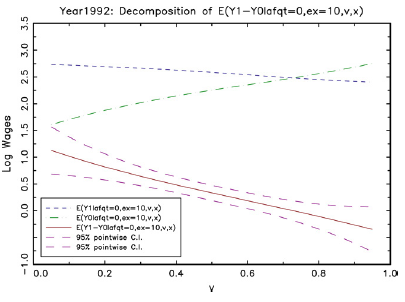
\includegraphics[width=\textwidth]{fig11_1}
\caption{Carneiro, Lee (2009)}
\end{subfigure}
\begin{subfigure}{0.5\textwidth}
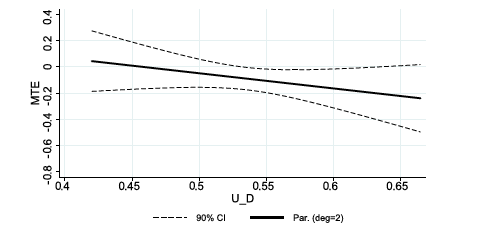
\includegraphics[width=\textwidth]{fig11_2}
\caption{Johnson, Taylor (2019)}
\end{subfigure}
\end{figure}
\end{mdframed}
%%%%%%%%%%%%%%%
\end{document}

